\documentclass{article}
\usepackage{tabularx}
\usepackage{amsmath}
\usepackage{here}
\usepackage{graphicx}
\usepackage[margin=2cm]{geometry}
\usepackage{cite}
\usepackage[final]{hyperref}
\usepackage{listings}
\hypersetup{
	colorlinks=true,
	linkcolor=blue,
	citecolor=blue,
	filecolor=magenta,
	urlcolor=blue         
}

\begin{document}

\title{TP02\\Introduction to CUDA}
\date{01/09/22}
\maketitle

\begin{abstract}
	In this practical work, we will see how to build a simple program using CUDA.
\end{abstract}


\section{Introduction}
First, we need to download the latest version of CUDA from the Nvidia website. To do so, go to \\https://developer.nvidia.com/cuda-downloads and install the SDK 12 for Windows (x86).\\
You'll find the source of the practical work by cloning this git repository:
\begin{lstlisting}
	https://github.com/robinfaurypro/GPGPU_ISIMA_2022-2023.git
\end{lstlisting}
If you already download the sources, you can just update your local repository to the latest commit. The CMakeLists file is stored into the TP02 folder. Open a terminal on your working folder and use this cmake command:
\begin{lstlisting}
	cmake -G "Visual Studio 16 2019" -A x64 ..
\end{lstlisting}
If everything is going well, you can compile and run the TP02 executable. The application is divided into two entity, the main executable and the gpgpu library. On the gpgpu library, and only here, you have access to CUDA command. CUDA files have the cu extension and they are compiled by nvcc.

\section{GPU properties}
In the gpgpu.h file, create a function "void GetGPGPUInfo();". This function will print some GPU properties. On this function you can create a cudaDeviceProp object and ask CUDA to fill it.
\begin{lstlisting}
	cudaDeviceProp cuda_propeties;
	cudaGetDeviceProperties(&cuda_propeties, 0);
\end{lstlisting}
The only property you need to print now is the maxThreadsPerBlock one but, you can explore the structure to better understand your device.

\section{Working in one dimension}
In this section we will generate a gray-scale image on the GPU. First, create a new function in the gpgpu library.
\begin{lstlisting}
	void GenerateGrayscaleImage(
		std::vector<uint8_t>& host_image_uint8, int32_t width, int32_t height);
\end{lstlisting}
On this function, create a vector of float and call it host\_image\_float. Fill this image with the content of the image passed by reference divided by 255. You can use the function std::transform from the standard library.\\
We can now work on the GPU with our image. We need to ask CUDA to duplicate the new image on the GPU. For that we will:
\begin{enumerate}
	\item Allocate some memory on the GPU by using cudaMalloc.
	\item Copy our buffer by using cudaMemcpy.
	\item Call a kernel to fill the image.
	\item Copy back the content to the host.
	\item Free the GPU buffer.
\end{enumerate}
\begin{lstlisting}
	float* device_image_float = nullptr;
	cudaMalloc(&device_image_float, host_image_int8.size() * sizeof(float));
	cudaMemcpy(
		device_image_float,
		host_image_float.data(),
		host_image_int8.size() * sizeof(float),
		cudaMemcpyHostToDevice);
	// Call to the kernel
	cudaMemcpy(
		host_image_float.data(),
		device_image_float,
		host_image_int8.size() * sizeof(float),
		cudaMemcpyDeviceToHost);
	cudaFree(device_image_float);
\end{lstlisting}
You can notice the extra flag to the cudaMemcpy to indicate the direction of the memory transfer. At this moment, the object host\_image\_uint8 and host\_image\_float are only editable by the host and the device\_image\_float only by the device.\\
We can now create a kernel to fill the device\_image\_float buffer. The \_\_global\_\_ keyword must be used in front of a function to create a kernel.
\begin{lstlisting}
	__global__ void kernel_gray(float* device_image_float) {
		int32_t index = blockIdx.x * blockDim.x + threadIdx.x;
		device_image_float[index] = device_image_float[index] + 0.5f;
	}
\end{lstlisting}
This kernel read an image from the input and write on the output the addition of the value and 0.5. You can call the kernel with this line of code:
\begin{lstlisting}
	kernel_gray <<<32*3, 1024 >>> (device_image_float);
\end{lstlisting}
Use a std::transform to convert back the buffer copied from the GPU into the host\_image\_uint8 image. Don't forget to multiply the result by 255. Save the result in a png.\\
\begin{figure}[H]
	\centering
	
\includegraphics[scale=0.2]{figures/gray_faild.png}
	\caption{Partial gray fill of an image}
\end{figure}
A CUDA kernel call need two values, the first one is the number of block and the second one the number of thread per block. As we can see here, we fill only the 32 first lines of the image. On the kernel call we can see the $32*3$ operation. 32 correspond to the number of lines and 3 to the number of channels and 1024 the number of pixel per line. In this case, threads index pixels per row and blocks index rows. Modify this numbers to fill the image. Be careful, the number of thread per block must not be above the maxThreadsPerBlock. Going above this value or read out of bound of the buffer will cause a segfault of the kernel.

\section{Working in two dimension}
Having the ability to compute one pixel indexed is a good step but it's better to have its coordinates. Fortunately, CUDA allow us to use the dim3 object into the kernel invocation.
\begin{lstlisting}
	dim3 threads(32, 32);
	dim3 blocks(32, 32);
	kernel_uv <<<blocks, threads >>> (device_image_float, width, height);
\end{lstlisting}
Because, my GPU have a maximal value of 1024 thread per block I choose to work on small 32 by 32 patches. My resolution is 1024x1024 so I choose to run 32 by 32 block of patches. Each kernel will write 3 values, one by channel.
\begin{lstlisting}
	__global__ void kernel_uv(float* image, int32_t width, int32_t height) {
		int32_t x = blockIdx.x * blockDim.x + threadIdx.x;
		int32_t y = blockIdx.y * blockDim.y + threadIdx.y;
		//...
	}
\end{lstlisting}
Like in the TP01, generate a image of the uv.

\begin{figure}[H]
	\centering
	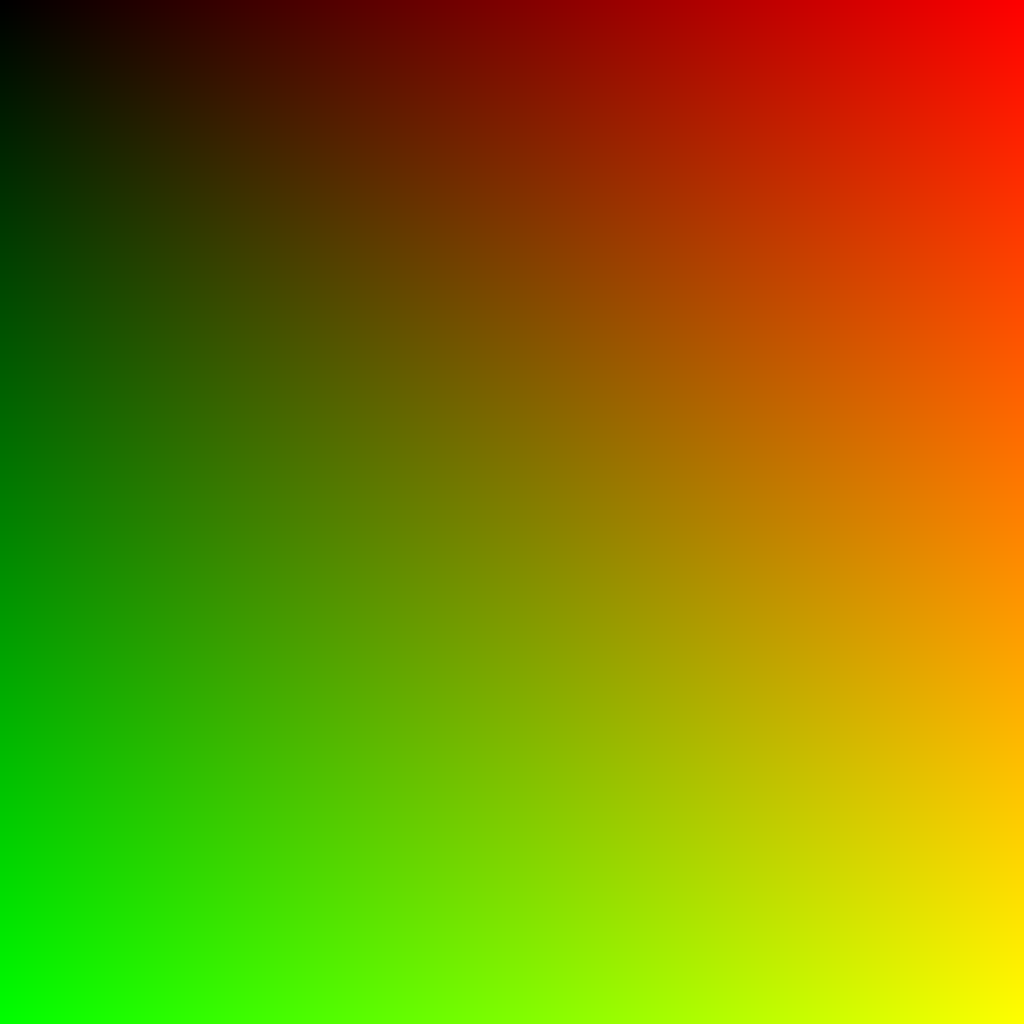
\includegraphics[scale=0.3]{figures/uv.png}
	\caption{UV of the image}
\end{figure}

\section{Working with heavy algorithm}
In this last section, we will run a heavy algorithm. Like the TP01, draw the Mandelbrot set. You can use some cuda funtions from cuComplex.h to work with complex number.
\begin{itemize}
	\item cuFloatComplex z = make\_cuFloatComplex(0.f, 0.f); to create a complex.
	\item cuCabsf to compute the absolute value of a complex.
	\item cuCaddf to add two complex.
	\item cuCmulf to multiply two complex.
\end{itemize}
In addition, the CUDA language support some basic algorithm like the min and max function. It's always a good idea to clamp the final result between 0 and 1.

\begin{figure}[H]
	\centering
	
\includegraphics[scale=0.35]{figures/Mandelbrot.png}
	\caption{Mandelbrot set}
\end{figure}


\end{document}